\begin{scanpage}{0158}{140}
\begin{center}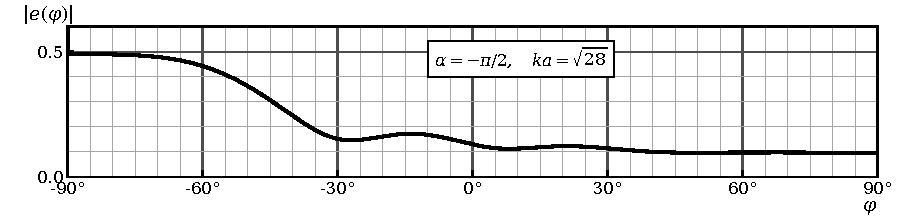
\includegraphics[width=.98\linewidth]{images/recreated/c-0158-fig57.pdf}\par
Figure 57. The same as Figure 55 when $\alpha=-\pi/2$.
\par\medskip
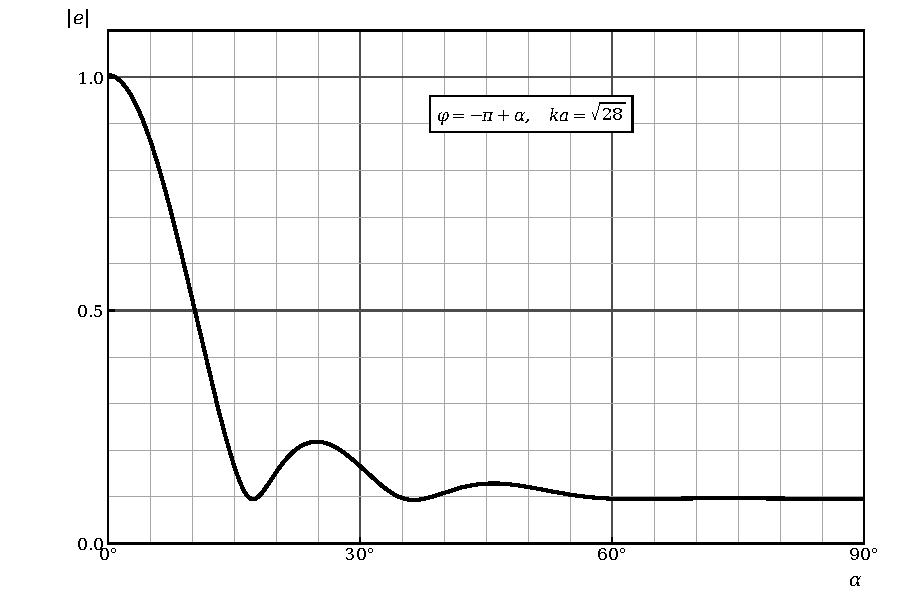
\includegraphics[width=.55\linewidth]{images/recreated/c-0158-fig58.pdf}\par
Figure 58. The same as Figure 55 when $\phi=-\pi+\alpha$.
\par\medskip
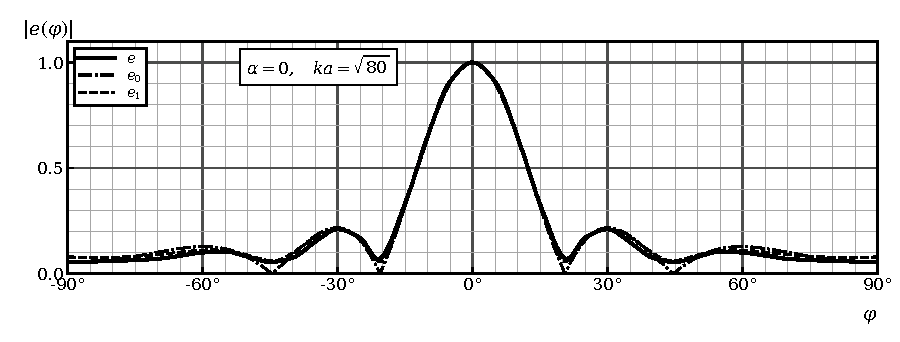
\includegraphics[width=.98\linewidth]{images/recreated/c-0158-fig59.pdf}\par
Figure 59. The function $e(\alpha,\phi)$ for a strip ($\alpha+0$, $ka=\sqrt{80}$). The electric vector is parallel to the strip's edge.
\end{center}
\end{scanpage}
